% !TEX root = ../probability_hse_exams.tex
\thispagestyle{empty}
\section{Решения контрольной номер 4. ИП}




\subsection[2018-2019]{\hyperref[sec:kr_04_ip_2018_2019]{2018-2019}}
\label{sec:sol_kr_04_ip_2018_2019}
\begin{enumerate}
\item
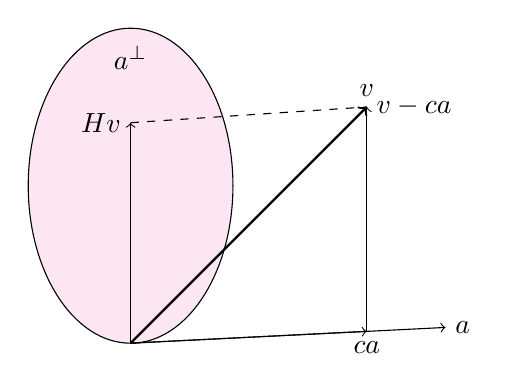
\begin{tikzpicture}
\filldraw[fill=magenta!10!white] (0,2) ellipse (1.3 and 2);
\draw (0, 3.9) coordinate [label = below:$a^{\perp}$];
\draw[->] (0,0) -- (4,0.2) node[right] {$a$};
\draw[->, thick] (0,0) -- (3,3) node[above] {$v$};
\draw[->] (0,0) -- (3,0.15) node[below] {$ca$};
\draw[->] (3,0.15) -- (3,3) node[right] {$v-ca$};
\draw[->] (0,0) -- (0,2.8) node[left] {$Hv$};
\draw[dashed] (0,2.8) -- (3,3);
\end{tikzpicture}

На рисунке вектор $ca$ по длине меньше вектора $a$ -- это необязательно так, данное предположение нужно, чтобы рисунок был. Вообще нам это неважно.
\begin{enumerate}
	\item
	Пусть есть некоторый вектор $v$. $ca$ -- его проекция на вектор $a$, где $c$ -- некоторая константа. Тогда $v - ca \perp a \Rightarrow \langle v - ca, a \rangle = 0$. Отсюда легко найти константу $c$: $\langle v,a \rangle - c \langle a, a \rangle = 0 \Rightarrow c = \frac{\langle v,a \rangle}{\langle a,a \rangle}$. $Hv$ -- проекция $v$ на $a^{\perp}$ по условию. По рисунку видно, что $Hv = v - ca$.
	
	Так как данное равенство верно для любого $v$, то мы можем рассмотреть вектора $(1,0,0)', (0,1,0)', (0,0,1)'$:
	\[
	\begin{pmatrix}
	h_1 & h_2 & h_3 \\
	h_4 & h_5 & h_6 \\
	h_7 & h_8 & h_9 \\
	\end{pmatrix}
	\begin{pmatrix}
	1 \\ 0 \\ 0
	\end{pmatrix}
	=
	\begin{pmatrix}
	1 \\ 0 \\ 0
	\end{pmatrix}
	-
	\frac{1}{9}
	\begin{pmatrix}
	1 \\ 2 \\ 2
	\end{pmatrix}
	\Rightarrow
	\begin{cases}
	h_1 = \frac{8}{9} \\
	h_4 = -\frac{2}{9} \\
	h_7 = -\frac{2}{9}
	\end{cases}
	\]
	Аналогично, находим остальные элементы матрицы:
	$\displaystyle
	H = \frac{1}{9}
	\begin{pmatrix}
	8 & -2 & -2 \\
	-2 & 5 & -4 \\
	-2 & -4 & 5 \\
	\end{pmatrix}$
	\item
	В общем виде:
	\[
	\begin{pmatrix}
	h_{11} & h_{12} & \ldots & h_{1n} \\
	h_{21} & \ldots & \ldots & \ldots \\
	\ldots & \ldots & \ldots & \ldots \\
	h_{n1} & \ldots & \ldots & h_{nn} \\
	\end{pmatrix}
	\begin{pmatrix}
	v_1 \\ v_2 \\ \ldots \\ v_n
	\end{pmatrix}
	=
	\begin{pmatrix}
	v_1 \\ v_2 \\ \ldots \\ v_n
	\end{pmatrix}
	-
	\frac{\langle v,a \rangle}{\langle a,a \rangle}
	\begin{pmatrix}
	a_1 \\ a_2 \\ \ldots \\ a_n
	\end{pmatrix}
	\]
	
	Запишем уравнение для 1 строки матрицы $H$:
	\[
	h_{11} v_1 + h_{12} v_2 + \ldots + h_{1n} v_n = v_1 - \frac{\langle v,a \rangle}{\langle a,a \rangle} a_1
	\]
	\[
	h_{11} v_1 + h_{12} v_2 + \ldots + h_{1n} v_n = \frac{(a_1^2 + a_2^2 + \ldots + a_n^2)v_1 - a_1(v_1 a_1 + v_2 a_2 + \ldots + v_n a_n)}{a_1^2 + a_2^2 + \ldots + a_n^2}
	\]
	
	Так как данное равенство верно для любого $v$, то коэффициенты при $v_i$ в обоих частях уравнения должны быть равны $\forall i$.
	
	Для $v_1$: $\displaystyle h_{11} = 1 - \frac{a_1^2}{a_1^2 + a_2^2 + \ldots + a_n^2} = \frac{a_1^2 + a_2^2 + \ldots + a_n^2 - a_1^2}{a_1^2 + a_2^2 + \ldots + a_n^2}$
	
	Для $v_2$: $\displaystyle h_{12} = -\frac{a_1a_2}{a_1^2 + a_2^2 + \ldots + a_n^2}$
	
	Обобщая написанное: $\displaystyle h_{ii} = \frac{a_1^2 + a_2^2 + \ldots + a_n^2 - a_i^2}{a_1^2 + a_2^2 + \ldots + a_n^2}; \,\, h_{ij} = \frac{-a_ia_j}{a_1^2 + a_2^2 + \ldots + a_n^2} \,\, \forall i \ne j$
	Теперь у нас достаточно данных, чтобы записать матрицу $H$.
	\item
	По условию $y$ - нормальный стандартный $n$-мерный вектор. Значит:
	\[
	\E(y) =
	\begin{pmatrix}
	0 \\ 0 \\ \ldots \\ 0
	\end{pmatrix};
	\,\,\,\,\,
	\Var(y) =
	\begin{pmatrix}
	1 & 0 & \ldots & 0 \\
	0 & 1 & \ldots & \ldots \\
	\ldots & \ldots & \ldots & \ldots \\
	0 & \ldots & \ldots & 1 \\
	\end{pmatrix}
	\]
	\item
	Заметим, что матрица $H$ симметрична. Из свойств матожидания и дисперсии:
	\[
	\E(Hy) = H \mathbb{E}(y) =
	\begin{pmatrix}
	0 \\ 0 \\ \ldots \\ 0
	\end{pmatrix};
	\,\,\,\,\,
	\Var(Hy) = H^T \Var(y) H = H^T H = H^2
	\]
	
	Можно также заметить, что проекция вектора, лежащего в $a^{\perp}$, на пространство $a^{\perp}$~-- это сам вектор: $H(Hv) = Hv \Rightarrow H^2 = H \Rightarrow \Var(Hy) = H$.
	\item
	По доказанному ранее: $y'Hy = y'HHy = y'H^THy = (Hy)^THy = ||Hy||^2 \sim \chi^2_{n-1}$. Известно, что квадрат длины проекции стандартного нормального вектора в пространство размерности $n-1$ распределен как хи-квадрат с $n-1$ степенями свободы.
\end{enumerate}
\end{enumerate}

\subsection[2017-2018]{\hyperref[sec:kr_04_ip_2017_2018]{2017-2018}}
\label{sec:sol_kr_04_ip_2017_2018}